\begin{question}
\emph{Hamming numbers} are numbers whose only prime factors are $2$, $3$,
and~$5$.  Hence the first few Hamming numbers are:
\[ \mstyle
1, 2, 3, 4, 5, 6, 8, 9, 10, 12, 15, 16.
\]
Thus each Hamming number is either~$1$, or an earlier Hamming number
multiplied by~$2$, $3$, or~$5$.

The Hamming numbers can be produced by a circuit as depicted below.
%
\begin{center}
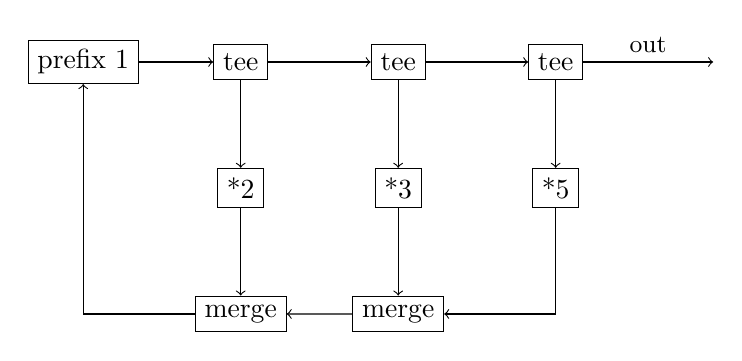
\begin{tikzpicture}[yscale = 0.8]
\draw (0,0) node[draw] (prefix) {\scalashape prefix 1};
% (*2) branch
\draw (prefix) ++ (2,0) node[draw] (tee2) {\scalashape tee};
\draw[->] (prefix) -- (tee2);
\draw (tee2) ++ (0,-2) node[draw] (mult2) {\scalashape *2};
\draw[->] (tee2) -- (mult2);
% (*3) branch
\draw (tee2) ++ (2,0) node[draw] (tee3) {\scalashape tee};
\draw[->] (tee2) -- (tee3);
\draw (tee3) ++ (0,-2) node[draw] (mult3) {\scalashape *3};
\draw[->] (tee3) -- (mult3);
% (*5) and out branch
\draw (tee3) ++ (2,0) node[draw] (tee4) {\scalashape tee};
\draw[->] (tee3) -- (tee4);
\draw (tee4) ++ (0,-2) node[draw] (mult5) {\scalashape *5};
\draw[->] (tee4) -- (mult5);
\draw[->] (tee4) -- node[above] {\small\scalashape out} ++ (2,0);
% merge of (*3) and (*5)
\draw (mult3) ++ (0,-2) node[draw] (merge1) {\scalashape merge};
\draw[->] (mult5) |- (merge1);
\draw[->] (mult3) -- (merge1);
% merge with (*2)
\draw (mult2) ++ (0,-2) node[draw] (merge2) {\scalashape merge};
\draw[->] (merge1) -- (merge2);
\draw[->] (mult2) -- (merge2);
% close loop
\draw[->] (merge2) -| (prefix);
\end{tikzpicture}
\end{center}
%
The |prefix 1| and |tee| components are as in Figure~\ref{fig:NatsCircuit}.
The |*2|, |*3|, and~|*5| components multiply their inputs by~$2$, $3$ and~$5$,
respectively.  The |merge| components receives two strictly increasing streams
and merges them together into a single strictly increasing stream; note that
this involves removing duplicate values, so this is slightly different from
the |merge| component we used in Section~\ref{sec:mergesort}.

Thus the |prefix 1| component sets things going; the |*2|, |*3|, and |*5|
components produce appropriate multiples; and the |merge| components merge the
streams together.

\begin{enumerate}
\item Implement the circuit using synchronous channels.  You will find that
  the system deadlocks.  Why is this?

\item Adapt the network to use buffered channels, where appropriate.  Is finite
  buffering enough?

\item Adapt the network so that it produces outputs only up to some given
  maximum value, and then terminates cleanly.
\end{enumerate}
\end{question}

%%%%%%%%%%%%%%%%%%%%%%%%%%%%%%%%%%%%%%%%%%%%%%%%%%%%%%%

\begin{answerI}
The |*2|, |*3|, and~|*5| components are simply instances of~|map|.

The |merge| function can be written as follows.  This meaintains the invariant
that  |l| is the last value read from |left|, and |r| is the last value read
from |right|.  In this example, closing of channels is just used to signal
termination, so we do not need to worry about outputting remaining inputs.
%
\begin{scala}
  def merge(left: ??[Int], right: ??[Int], out: !![Int]) = thread("Merge"){
    var l = left?(); var r = right?()
    repeat{
      if(l < r){ out!l; l = left?() }
      else if(l == r){ out!l; l = left?(); r = right?() }
      else{ out!r; r = right?() }
    }
    left.close(); right.close(); out.endOfStream()
  }
\end{scala}

The following function produces the system (including the latter part of the
question).
%
\begin{scala}
def system(out: !![Int], max: Int) = {
  val h0, h1, h2 = new SyncChan[Int]     // Inputs into £tee£ components.
  val i2, i3, i5 = new SyncChan[Int]     // Inputs into £*2£, £*3£, £*5£.
  val t2, t3, t5 = new UnboundedBuffChan[Int] // Outputs from £*2£, £*3£, £*5£.
  val m1, m2, m3 = new SyncChan[Int]    // Outputs from £merge£s and £takeWhile£.
  prefix(1, m3, h0) || tee(h0, i2, h1) || tee(h1, i3, h2) || tee(h2, i5, out) ||
  map((x:Int) => 2*x, i2, t2) || map((x:Int) => 3*x, i3, t3) || 
  map((x:Int) => 5*x, i5, t5) ||  
  merge(t2, t3, m1) || merge(t5, m1, m2) || 
  takeWhile((x: Int) => x <= max, m2, m3)
}
\end{scala}

The system without buffering deadlocks, basically because there are too many
intermediate values passing round the system for the various components to
hold.  In a bit more details, suppose the |prefix| component has just passed
a value~$n$.  Then the |*2| component will have output most of the Hamming
numbers less than $2n$; I say ``most'', because there might be a couple of
Hamming numbers either still in the |*2| component or the previous |tee|
component.  But that means that most of the Hamming numbers between $n$
and~$2n$ have to be stored somewhere in the subcircuit between the |*2| and
|prefix| components---and there simply isn't enough capacity for all of them. 
 
I use a buffered channel for the output from the |*2| component to store
them.  In fact, the number of Hamming numbers between~$n$ and~$2n$ tends to
infinity as $n$ tends to infinity, so we need an unbounded buffer.  The same
is true for the |*3| and |*5| components. 

To achieve termination, I inserted a |takeWhile| component just before the
|prefix| component---but it could have been inserted pretty much anywhere.
Also, each component is adapted to close its output channels when its main
loop terminates, and also arrange for the |takeWhile| and |merge| components
to close their input channels; the latter is necessary, or else we can get
into a situation where one of those components is trying to send to another,
but the latter has terminated, so the network is deadlocked.  There's no harm
in \emph{every} component closing its input channels.
\end{answerI}
